\documentclass[12pt]{article}%
\usepackage{hyperref}
\usepackage{listings}
\usepackage{color}
\usepackage{multicol}
\usepackage{amsfonts}
\usepackage{fancyhdr}
\usepackage{comment}
\usepackage[a4paper, top=2.2cm, bottom=2.2cm, left=2.2cm, right=2.2cm]%
{geometry}
\usepackage{times}
\usepackage{changepage}
\usepackage{amssymb}
\usepackage{graphicx}%
\newtheorem{theorem}{Theorem}
\newtheorem{acknowledgement}[theorem]{Acknowledgement}
\newtheorem{algorithm}[theorem]{Algorithm}
\newtheorem{axiom}{Axiom}
\newtheorem{case}[theorem]{Case}
\newtheorem{claim}[theorem]{Claim}
\newtheorem{conclusion}[theorem]{Conclusion}
\newtheorem{condition}[theorem]{Condition}
\newtheorem{conjecture}[theorem]{Conjecture}
\newtheorem{corollary}[theorem]{Corollary}
\newtheorem{criterion}[theorem]{Criterion}
\newtheorem{definition}[theorem]{Definition}
\newtheorem{example}[theorem]{Example}
\newtheorem{exercise}[theorem]{Exercise}
\newtheorem{lemma}[theorem]{Lemma}
\newtheorem{notation}[theorem]{Notation}
\newtheorem{problem}[theorem]{Problem}
\newtheorem{proposition}[theorem]{Proposition}
\newtheorem{remark}[theorem]{Remark}
\newtheorem{solution}[theorem]{Solution}
\newtheorem{summary}[theorem]{Summary}
\usepackage{commath}
\usepackage{url} 
\usepackage{hyperref}
\usepackage[style=numeric]{biblatex}
\usepackage{subfig}
\usepackage{minted}
% \usepackage[utf8]{inputenc}
% \usepackage[english]{babel}
\usepackage{esvect}
\addbibresource{reference.bib}


\usepackage{commath}

\newenvironment{proof}[1][Proof]{\textbf{#1.} }{\ \rule{0.5em}{0.5em}}
\usepackage[utf8]{inputenc}

% \usepackage{algorithm}
% \usepackage{algorithmic} %format of the algorithm


% Default fixed font does not support bold face
\DeclareFixedFont{\ttb}{T1}{txtt}{bx}{n}{12} % for bold
\DeclareFixedFont{\ttm}{T1}{txtt}{m}{n}{12}  % for normal

\usepackage{graphics}

% Custom colors
\usepackage{color}
\definecolor{deepblue}{rgb}{0,0,0.5}
\definecolor{deepred}{rgb}{0.6,0,0}
\definecolor{deepgreen}{rgb}{0,0.5,0}

\usepackage{listings}
\newcommand{\Q}{\mathbb{Q}}
\newcommand{\R}{\mathbb{R}}
\newcommand{\C}{\mathbb{C}}
\newcommand{\Z}{\mathbb{Z}}

% Python style for highlighting
\newcommand\pythonstyle{\lstset{
language=Python,
basicstyle=\ttm,
otherkeywords={self},             % Add keywords here
keywordstyle=\ttb\color{deepblue},
emph={MyClass,__init__},          % Custom highlighting
emphstyle=\ttb\color{deepred},    % Custom highlighting style
stringstyle=\color{deepgreen},
frame=tb,                         % Any extra options here
showstringspaces=false            % 
}}

% Python environment
\lstnewenvironment{python}[1][]
{
\pythonstyle
\lstset{#1}
}
{}

% Python for external files
\newcommand\pythonexternal[2][]{{
\pythonstyle
\lstinputlisting[#1]{#2}}}
\usepackage[utf8]{inputenc}
\usepackage{amsmath, nccmath}
\usepackage{geometry}

\usepackage{algorithm}
\usepackage{arevmath}     % For math symbols
\usepackage[noend]{algpseudocode}

\begin{document}

\title{Institute of Robotics,  University of Innopolis}
\author{Computational Intelligence \\ Subspaces and Projection}
\date{\today}
\maketitle


\section{Four Fundamental Subspaces}

\subsection{Task 01}

Let A be $\begin{bmatrix}
2 & -1 & -3\\ 
 -4 & 2 & 6
\end{bmatrix}$. Calculate $C(A), N(A), C(A^T),$ and $N(A^T)$, then show that 
\begin{enumerate}
     \item Any member of row space is orthogonal to any member of nullspace
    \item Any member of column space is orthogonal to any member of left nullspace
\end{enumerate}

You may use null(A) and colspace(sym(A)) to calculate those listed above. 

\begin{figure}[h]%
    \centering
\subfloat[\centering ?]{{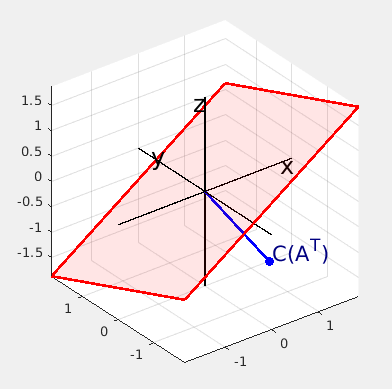
\includegraphics[width=5cm]{row_null.png} }}%                                                                                                                           
    \qquad
    \subfloat[\centering ?]{{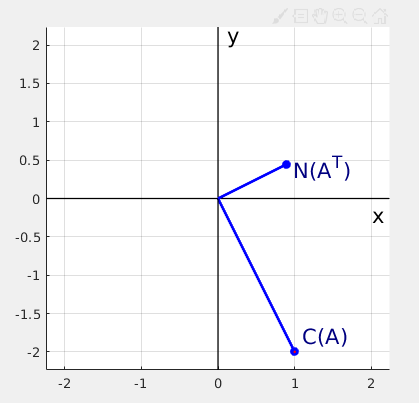
\includegraphics[width=5cm]{left_null_col.png} }}%
    % \caption{2 Figures side by side}%
    \label{fig:example}%
\end{figure}

% \begin{minted}
% [
% frame=lines,
% framesep=2mm,
% baselinestretch=1.2,
% ]
% {matlab}
% a =  [2 -1 -3; -4 2 6];

% col_space = double(colspace(sym(a)));
% row_space = double(colspace(sym(a')));
% left_null_space = null(a');
% null_space = null(a);

% figure(1); clf; hold on;
% drawVector(row_space, {'C(A^T)'});
% drawSpan(null_space, 'r');

% figure(2); clf; hold on;
% drawVector(col_space, {'C(A)'});   
% drawVector(left_null_space, {'N(A^T)'});
% \end                                                                                                                                                                                                                                                                                                                                                                                                                                                                                                                                                                                                                                                                                                                                                                                                                                                                                                                                                                                                                                                                                                                                                                                                                                          {minted}
 \begin{figure}[h]
\begin{center}
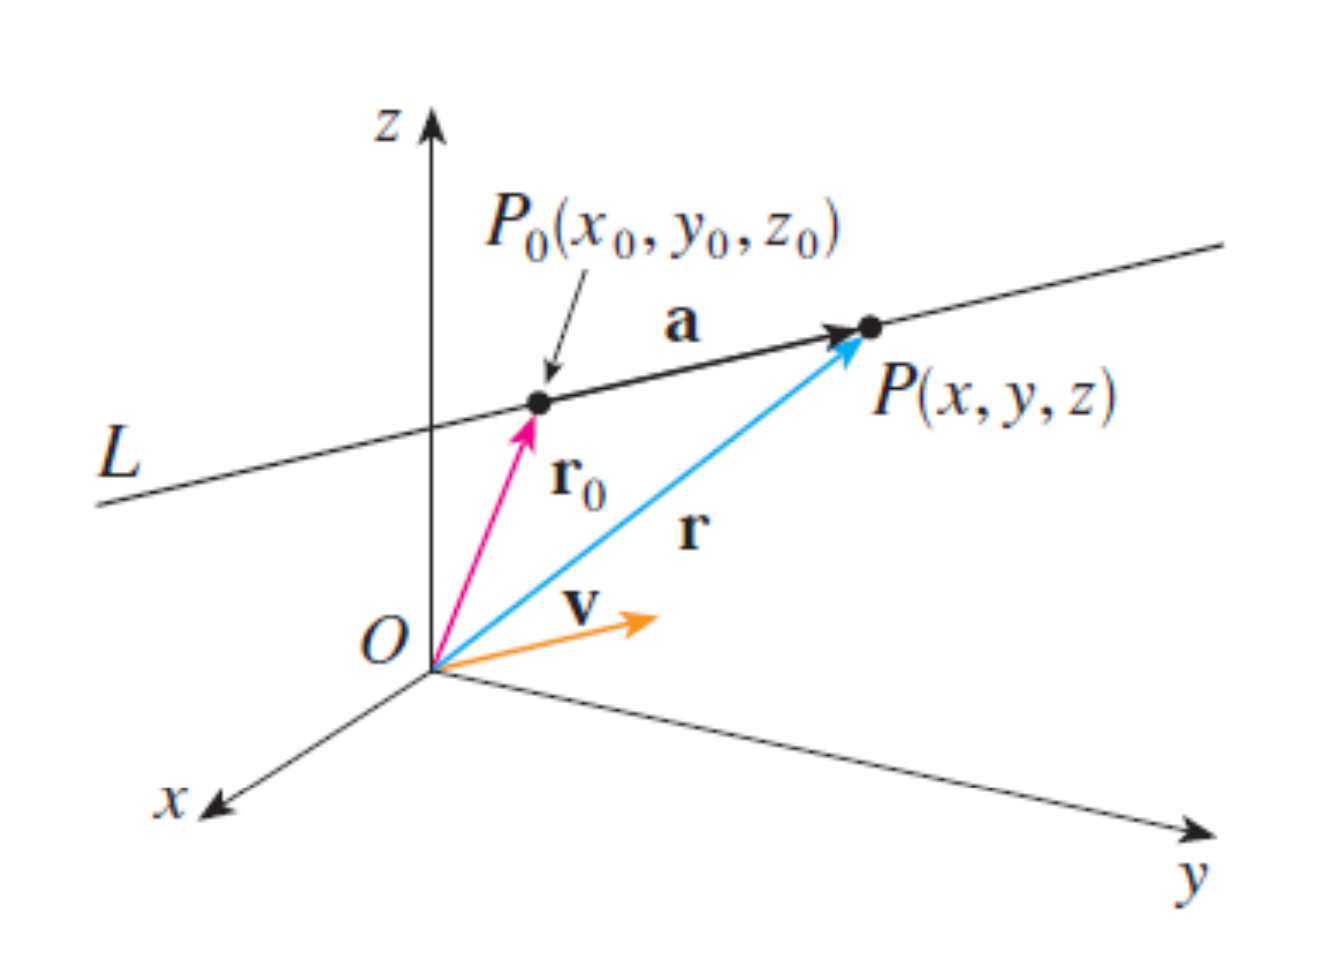
\includegraphics[width=7cm, height=6cm]{line_3d.png}
\caption{}\label{fig:l                                                                                                                                                                                                                                                                                                                                                                                                                                                                                                                                                                                                                                                                                                                             ine}
\end{center}
\end{figure}



\subsection{Task 02}
A line containing the point $P_0= x_0,y_0,z_0$ and parallel to the vector $\mathbf{v}=<a,b,c>$ can be described in the form of parametric equations

 \begin{figure}[h]
\begin{center}
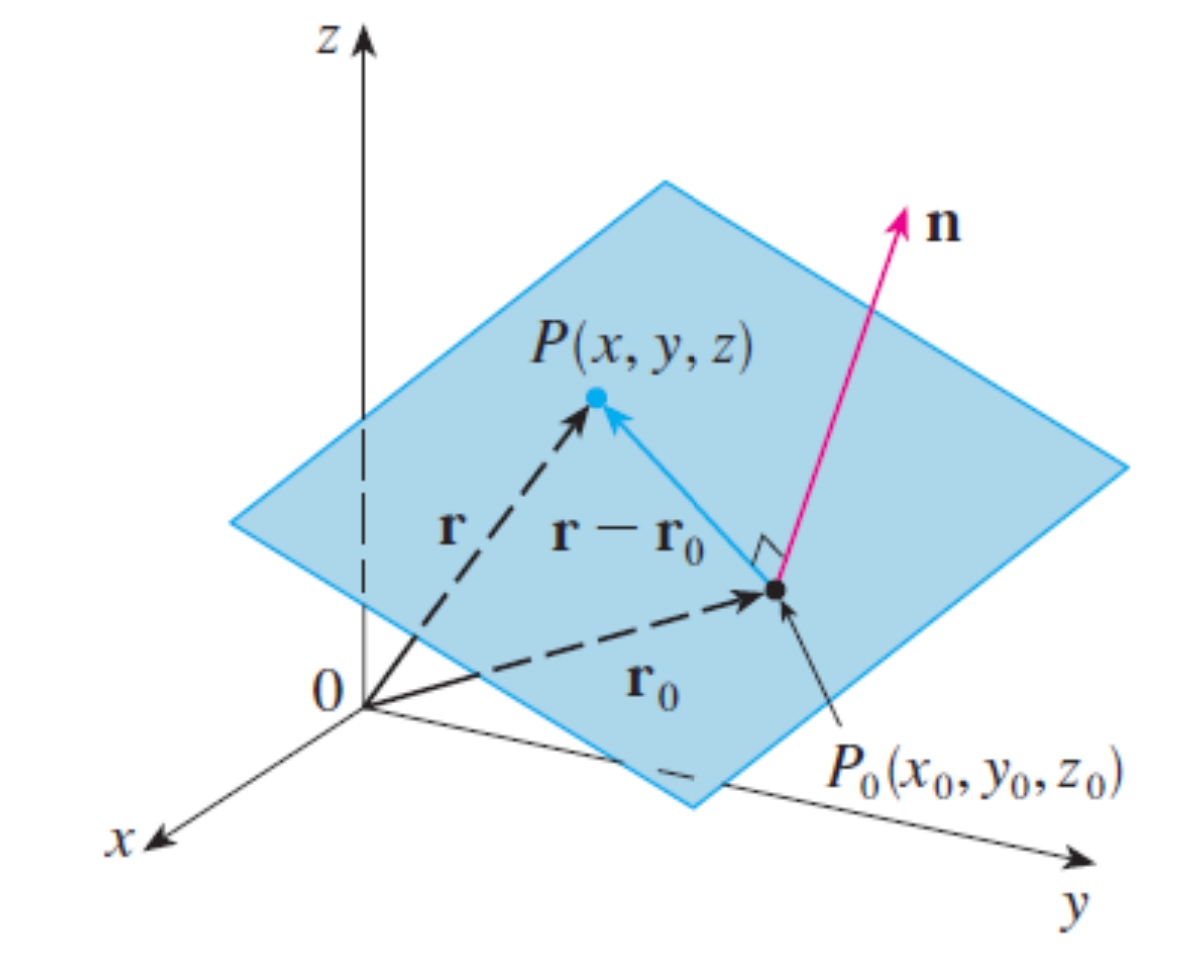
\includegraphics[width=7cm, height=6cm]{3d_plane.png}
\caption{}\label{fig:plane}
\end{center}
\end{figure}


\begin{enumerate}
    \item By looking at Figure~\ref{fig:line}, define the parametric equations of a line?
    \item If two lines, i.e., $\mathbf{r_1} = p_1 + t_1\mathbf{v_1}$ and  $\mathbf{r_2} = p_2 + t_2\mathbf{v_2}$, are intersect each other, how can you verify it?
    %null(v1 -v2)
\end{enumerate}

\subsection{Task 03}
A plane can be described by $\mathbf{n}\cdot (\mathbf{r}-\mathbf{r_0}) = 0$ where $\mathbf{n} = <a,b,c>$ (normal vector) and $\mathbf{r_0} = <x_0,y_0,z_0>$ (position vector), refer to Fig.\ref{fig:plane}

\begin{enumerate}
    \item If two planes, i.e., $\mathbf{r_1} = p_1 + t_1\mathbf{v_1} + u_1\mathbf{w_1}$ and  $\mathbf{r_2} = p_2 + t_2\mathbf{v_2} + u_2\mathbf{w_2}$, are intersect each other, how can you verify it?
    %null(d1 -d2)
    \item Find the equation of the plane passing through origin if following two vectors are in the same plane, $\mathbf{v_1}=<1, -5, 1>$ and $\mathbf{v_2}=<2,-1,-5>$
    %n = null([v_1 v_2]^T) = cross(v_1, v_2)
    
    \item Given $\mathbf{n}$ (or normal vector) how can you formulate the corresponding plane equation in the vector form?
    % [d1 d2 ] = null(n^T)
\end{enumerate}



\section{Projection}


\subsection{Task 01}
\begin{enumerate}
    \item Let's consider in 2D and higher dimensional projections separately. With help of Fig.\ref{f:prjection}, try to prove $p$ is given by $a\frac{a^Tb}{a^Ta}$. If the projection matrix is defined by $p =Pb$, show that $P = \frac{aa^T}{a^Ta}$. With that, we can define $A\hat{x} = p$ where we can find an approximate solution, i.e., $\hat{x}$
    \item If $a_1$ and $a_2$ form a basis for the plane, and $A = [a_1 \; a_2]$, show that projection is given by $P = A(A^TA)^{-1}A^T$
    \item How can we find the projection onto row space of A? 
    % (column space of $A^T$)
    
    \item What can you say about $P^T, P$ and $P^2, P$, if A does happen to be square, invertible matrix?

\end{enumerate}
 
\subsection{Task 02} 
Let $A$ be $\begin{bmatrix}
1 & 1\\ 
 2 & 1\\ 
 -1 & -1 \\ 
-2 & -1
\end{bmatrix}$.

\begin{enumerate}
    \item Find the $A^{+}$ (left inverse of A)?
    \item The projection onto the column space of A?
    %AA^{+}
    \item The projection onto the left nullspace of A (orthogonal complement of the column space)?
    %I-AA^{+}
\end{enumerate}

\subsection{Task 03}
$V = \{\mathbf{x} = \begin{bmatrix}
x\\ 
y\\ 
z
\end{bmatrix} \in R^3 \mid x + y + z = 0 \} = span
\left (
\begin{bmatrix}
-1\\ 
1\\ 
0
\end{bmatrix},\begin{bmatrix}
-1\\ 
0\\ 
1
\end{bmatrix}  \right ) $
\begin{enumerate}
    \item  What does N(V) represent?
    \item How can we find the projection of any vector in $\mathbb{R}^3$ on to V, namely $Proj_V \mathbf{x}$?
    %Proj_V \mathbf{x} = A(A^{+})x
    \item How can we find the orthogonal complement of V  ($V^{\perp}$)
     %I-AA^{+}
     \item How can we find the projection of any vector in $\mathbb{R}^3$ on to $V^{\perp}$, namely $Proj_{V^{\perp}} \mathbf{x}$? 
     % same as before question
     \item Find the projection that all $\mathbf{x}$s are not in the V?
     %$Proj_{V^{\perp}}
\end{enumerate}

\subsection{Task 04}
Consider the following system:
\begin{equation}\label{eq:system}
    \dot{x} = f(x) = Ax, \; x(0) = x_0
\end{equation}, where $x\in \mathbb{R}^n$ and $t \geq 0$. Let $x^* = \Theta(t_0,x^*)$ be an equilibrium point at $t_0$ for the considered system (\ref{eq:system}). Such a $x^*$ said to be stable (in the sense of Lyapunov)~\cite{ronbun} if and only if for a given $\epsilon > 0$, there exists a $\delta(t_0, \epsilon) >0$ such that 
\begin{equation}
    \left \|  \Theta(t_0,x^*) \right \| \leq \delta \Rightarrow \left \| \Theta(t,x^*) \right \| < \epsilon, \; \forall t \leq t_0.
\end{equation} and said to be attractive (in the sense of Lyapunov) if and only if there exists $\delta (t_0)$ such  that:
\begin{equation}
    \left \| \Theta(t_0,x^*)\right \| \leq \delta \Rightarrow \lim_{t\rightarrow inf} \left \| \Theta(t_0,x^*) \right \| = 0.
\end{equation}Along with that, considered system is asymptotically stable (sense of Lyapunov) if the system is stable and attractive. Let $V(x) = x^TPx$, where $P$ is a positive definite matrix, be a Lyapunov function for the system (\ref{eq:system}). If the system is stable if there exists a P:
\begin{equation}
    \dot{V}(x) = (Ax)^TPx + x^TPAx \; = -x^TQx
\end{equation}Thus, Lyapunov conditions can be written as 
\begin{equation}
    \begin{aligned}
      P >0 \\
      A^TP + PA + Q = 0
    \end{aligned}
\end{equation}

Lyapunov equations for a continuous system has form: $A^TP + PA  =-Q$. As long as there exists such positive definite $P$ that Lyapunov equations holds for a positive definite $Q$, the system is stable. You are given the following information about system
\begin{equation}
    \begin{aligned}
      Q = \begin{bmatrix}
1 & 0 \\ 
 0& 1
\end{bmatrix}, \; A = \begin{bmatrix}
-10 & 5\\ 
 -5 & -10
\end{bmatrix}
    \end{aligned}
\end{equation} Check whether system is stable or not? These APIs may help
\begin{minted}
[
frame=lines,
framesep=2mm,
baselinestretch=1.2,
]
{matlab}
#Python
scipy.linalg.solve_continuous_lyapunov
scipy.linalg.solve_discrete_lyapunov
scipy.linalg.eig
#Matlab
lyap(A,Q)
dlyap(A,Q)
eig(X)

\end{minted}

Now let's consider 
\begin{equation}
    \begin{aligned}
      A = \begin{bmatrix} -10.05 & -0.021 & -0.02 \\  
0 & 0 & 0 \\  
-0.022 & 0.0032 & -10.055
\end{bmatrix}
    \end{aligned}
\end{equation} where system state is defined by $x = x_1,x_2, x_3$. Let's denote the value of $x_2$ as c since $x_2$ is a constant. Can you rewrite the system in terms of remaining variables $x_1$ and $x_3$ and prove its stability using the Lyapunov equation? 

Orthonormal basis in the column space of the state matrix in this case is:

$$
C =
\begin{pmatrix} 
1 & 0 \\  
0 & 0 \\  
0 & 1
\end{pmatrix}
$$

Motion of the system takes place in that column space. Let's denote $y = C^{\top}x$, and as long as $x$ is in this column space, it is true that $x = Cy$. But if $x$ is not in the column space, it is $x = Cy + x^*$

Notice that $x^*$ is in the left null space of the state matrix, as long as $y = C^{\top}x$, because: 

$$Cy = CC^{\top}x$$
$$x-x^* = CC^{\top}x$$
$$x^* = (I-CC^{\top})x$$

where the last expression is a projection of $x$ onto the left null space of the state matrix. Orthonormal basis in the left null space of the state matrix is:

$$
L =
\begin{pmatrix} 
0 \\  
1 \\  
0
\end{pmatrix}
$$

And we know that $x_2 = c$, so $x^* = Lc$.

Variable $y$ is the new coordinates in the column space basis.

Let's project the dynamics into the column space. First we multiply it by $C^{\top}$:

$$C^{\top} \dot x = 
C^{\top}
\begin{pmatrix} -10.05 & -0.021 & -0.02 \\  
0 & 0 & 0 \\  
-0.022 & 0.0032 & -10.055
\end{pmatrix}
x
$$

$$\dot y = 
\begin{pmatrix} -10.05 & -0.021 & -0.02 \\ 
-0.022 & 0.0032 & -10.055
\end{pmatrix}
x
$$

Then, since $x = Cy + Lc$ on the system trajectory, we get:

$$\dot y = 
\begin{pmatrix} -10.05 & -0.021 & -0.02 \\ 
-0.022 & 0.0032 & -10.055
\end{pmatrix}
(Cy + Lc)
$$

$$\dot y = 
\begin{pmatrix} -10.05 & -0.02 \\ 
-0.022 & -10.055
\end{pmatrix}
y
+
\begin{pmatrix} 
-0.021 \\ 
0.0032
\end{pmatrix}
c
$$

From here you apply Lyapunov eq. directly.

\section{Appendix 1}

Let $A$ be a $m\times n$ matrix, then four sub spaces cab be defined as follows:
\begin{enumerate}
    \item The column space $C(A) \in \mathbb{R}^m$, Its dimension is the Rank(A) = r  
    \item The nullspace $N(A) \in \mathbb{R}^n$, Its dimension is the Rank(A) = n - r  
    \item The row space $C(A^T) \in \mathbb{R}^n$, Its dimension is the Rank(A) = r  
    \item The left nullspace $N(A^T) \in \mathbb{R}^m$, Its dimension is the Rank(A) = r-m  
\end{enumerate} The relationships among the fundamental subspaces are shown in Fig.~\ref{f:sub_spaces}.

\begin{figure}[!ht]
\begin{center}
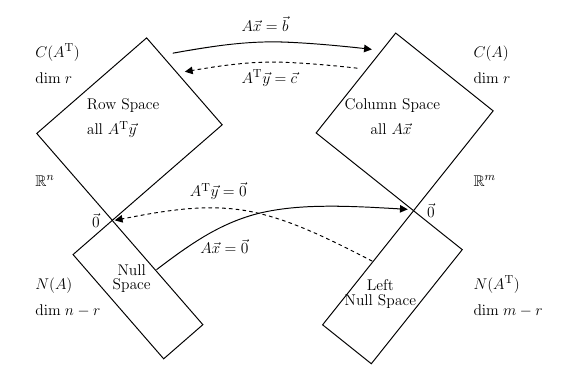
\includegraphics[width=10cm]{sub_spaces.png}
\caption{\label{f:sub_spaces} The fundamental subspaces~\cite{rose1982linear}}
\end{center}
\end{figure} 

\subsection{Let's get to the point}\label{sec:vector_space}
Get back to the basic and see how we can solve Least-squares problem using linear algebra rather than using calculus. To get things clear, Let me formulate the problem in a bit different form. 
\begin{equation}\label{col_space}
   \underbrace{\begin{bmatrix}
1 & 0\\ 
5 & 4\\ 
2 & 4
\end{bmatrix}}_A\underbrace{\begin{bmatrix}
x\\ 
y
\end{bmatrix}}_{\mathbf{x}} = \underbrace{\begin{bmatrix}
b_1\\ 
b_2
\\ 
b_3
\end{bmatrix}}_b
\end{equation} where $\mathbf{x} = [x \; y]^T$. In Eq.~\ref{col_space}, the relationship between three points in  $\mathbb{R}^2$ is given. If you are given $b_1, b_2,$ and $b_3$ can you try to find the solution for $x$ and $y$? If there is exist a combination of columns of A that can be form exactly equal to b. In other words, to hold preceding condition b should be in the same column space where A's columns are belonged.  Let's try to visualize and see in which condition should hold in order to b lies in the same column space, i.e., C(A).

% \begin{figure}[!ht]
% \begin{center}
% 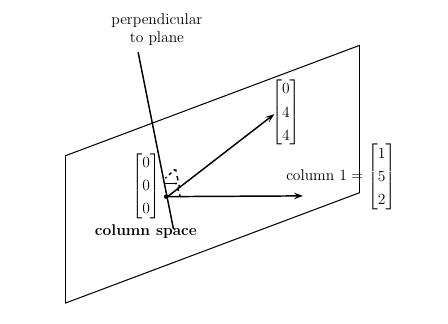
\includegraphics[width=9cm]{colspace.png}
% \caption{\label{f:colspace} The column space of A, i.e., C(A)~\cite{rose1982linear}}
% \end{center}
% \end{figure} 

\begin{figure}%
    \centering
    \subfloat[\centering \label{f:colspace} The column space of A, i.e., C(A)~\cite{rose1982linear}]{{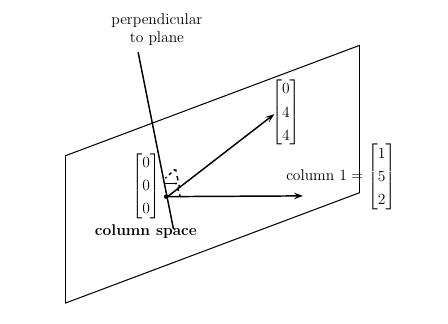
\includegraphics[width=7cm]{colspace.png} }}%
    \qquad
    \subfloat[\centering\label{f:prjection} Projection b on a]{{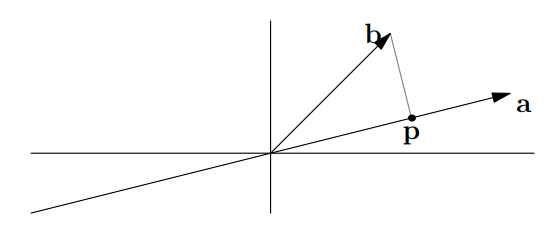
\includegraphics[width=8cm]{plane_.png} }}%
    \label{fig:example}%
\end{figure}

When will b be either or both $x$ and $y$ equal to zero? Thus, $Ax = b$ can be solved if and only if b lies in the plane where columns of A lie or C(A). If $b=0$ can you try to solve, $Ax=0$? The solution to $Ax=0$ form another vector space which we called the null space of A, i.e., N(A). So in this case, define the vectors that are belonged to N(A)? %only 0,0%
As we discussed, there is no exact solution for when $b$ does not lie on the C(A). Hence,to solve these kind of problems we have to to find the projection b onto the C(A). In other word, projections gives the minimum error to b. 


\subsection{Homogeneous coordinates and some geometric primitives}
A point (X) in $\mathbb{R}^3$  is presented by a vector with 4 entries in homgeneous representation, i.e.,  $x=<x_1, x_2, x3_, x4>$, where $x_4 \neq 0$. On the contrary, a point in $\mathbb{R}^3$, i.e., (x,y,z), what would be the homogeneous representation? Besides, the projective transformation on $\mathbb{P}^3$ can be defined as: $X^{'} = HX$ where $H$ is a linear transformation operator? 

\subsubsection{Points and Planes in 3D}
A plane in $\mathbb{R}^3$ can be written as $P = aX+bY+cZ+d = 0$ with homogeneous representation $\mathbf{P} = (a,b,c,d)^T$ in $\mathbb{P}^3$. If a given point $\mathbf{X} = (x,y,z,1)^T$ lies on P then $\mathbf{X}^T\mathbf{P} = 0$ or $\mathbf{P}^T\mathbf{X} = 0$. Now consider a set of n points are stacked into a single matrix as 
    \begin{equation}
        A = \begin{bmatrix}
\mathbf{X}^{1T}\\ 
\mathbf{X}^{2T}\\ 
\vdots \\ 
\mathbf{X}^{nT}
\end{bmatrix} \in \mathbb{R}^{n\times 4}.
    \end{equation} Based on the rank(A), configuration of the set of points can be described: Fig.~\ref{f:rank_4}, Fig.~\ref{f:rank_3}, Fig.~\ref{f:rank_2} and Fig.~\ref{f:rank_1}. Similarly, a set of n planes are stacked into a single matrix as 
    \begin{equation}
        \pi = \begin{bmatrix}
\mathbf{P}^{1T}\\ 
\mathbf{P}^{2T}\\ 
\vdots \\ 
\mathbf{P}^{nT}
\end{bmatrix} \in \mathbb{R}^{n\times 4}.
    \end{equation} Based on the rank($\pi$), configuration of the set of planes can be described: Fig.~\ref{f:rank_4}, Fig.~\ref{f:rank_3}, Fig.~\ref{f:rank_2} and Fig.~\ref{f:rank_1}
    
    \begin{figure}[H]
    \begin{center}
    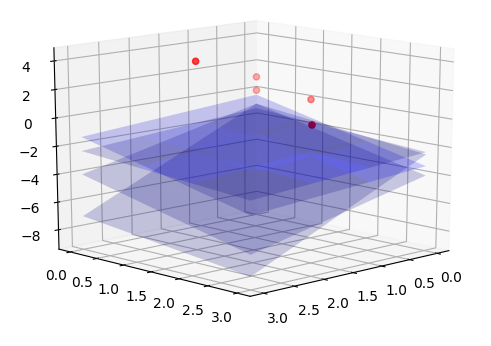
\includegraphics[width=7cm]{rank_4.png}
    \caption{\label{f:rank_4} When rank(A) is 4 what will be the dimension of N(A)? or rank($\pi$) is 4 what will be the dimension of N($\pi$)?}
    \end{center}
    \end{figure} 
    
    \begin{figure}[H]
    \begin{center}
    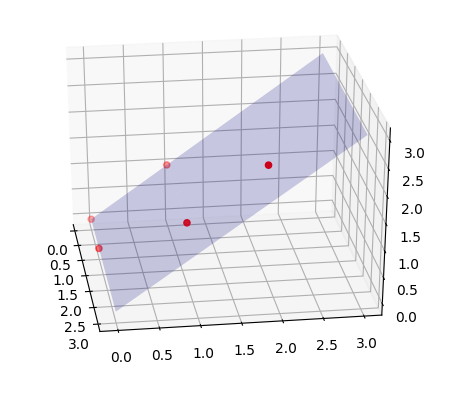
\includegraphics[width=7cm]{rank_3.png}
    \caption{\label{f:rank_3} For rank(A) = 3, N(A) describes a plane that points lie on or for rank($\pi$) = 1, N($\pi$) describes three points on planes}
    \end{center}
    \end{figure}
    
     \begin{figure}[H]
    \begin{center}
    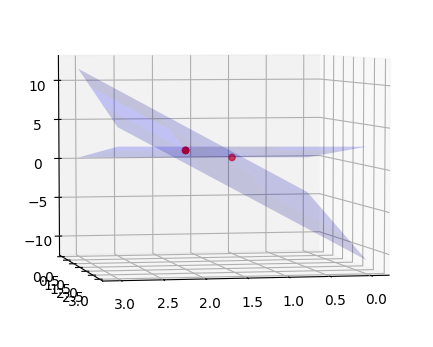
\includegraphics[width=7cm]{rank_2.png}
    \caption{\label{f:rank_2} For rank(A) = 2, N(A) describes two planes intersecting at line that points lie on or for rank($\pi$) = 2, N($\pi$) describes two points in 3D line at intersection of planes}
    \end{center}
    \end{figure}
    
    \begin{figure}[H]
    \begin{center}
    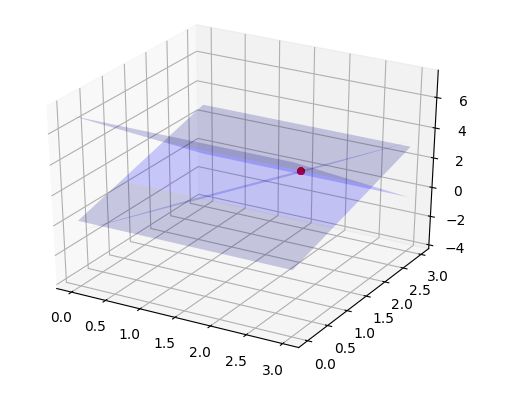
\includegraphics[width=7cm]{rank_1.png}
    \caption{\label{f:rank_1} For rank(A) = 1, N(A) describes three planes intersecting at points or for rank($\pi$) = 3, N($\pi$) describes a point that intersection of planes }
    \end{center}
    \end{figure}
\begin{minted}
[
frame=lines,
framesep=2mm,
baselinestretch=1.2,
]
{python}
from numpy.linalg import svd
import numpy as np
import matplotlib.pyplot as plt
from mpl_toolkits.mplot3d import Axes3D

def rank(A, atol=1e-13):
    s = svd(A, compute_uv=False)
    rank = int((s >= atol).sum())
    return rank

def nullspace(A, atol=1e-13):
    _, s, vh = svd(A)
    nnz = (s >= atol).sum()
    ns = vh[nnz:].conj().T
    return ns

A = np.array([[2, 2, 2, 1], [4, 2, 2, 2], [4, 1, 1, 4]
, [1, 4, 4, 4], [1, 1, 1, 2]])
# A = np.array([[2, 2, 2, 1], [2, 2, 2, 1], [4, 1, 1, 4]
# , [4, 1, 1, 4], [4, 1, 1, 4]])
# A = np.array([[2, 2, 2, 1], [2, 2, 2, 1], [2, 2, 2, 1]
# , [2, 2, 2, 1], [2, 2, 2, 1]])
# A = np.array([[2, 1, 4, 1], [2, 3, 1, 1], [2, 3, 2, 3]
# , [2, 1, 2, 4], [2, 1, 4, 4]])

plane_ = nullspace(A)

xx, yy = np.meshgrid(range(4), range(4))
zz = [(-plane_[:,i][0]*xx - plane_[:,i][1]*yy - plane_[:,i][3])
                *1./plane_[:,i][2] for i in range(0, plane_.shape[1])]
if(plane_.shape[1]==0):
    zz = [(-A[:,i][0]*xx - A[:,i][1]*yy - A[:,i][3])*1./A[:,i][2] 
            for i in range(0, A.shape[1])]
zz = np.array(zz)

plt3d = plt.figure()
ax = plt3d.add_subplot(111, projection='3d')
for i in range(0, zz.shape[0]):
    ax.plot_surface(xx, yy, zz[i], color='blue', alpha=0.2)
ax.scatter(A[:,0]/A[:,3], A[:,1]/A[:,3], A[:,2]/A[:,3]
                                    , marker='o', color="red")
plt.show()

\end{minted}

\printbibliography
\end{document}